%%% -*- mode: LaTeX/P; flyspell-mode: 1; -*-
%%% Time-stamp: <2024-04-20 12:04:08 vladimir>
%%% Copyright (C) 2019-2024 Vladimir G. Ivanović
%%% Author: Vladimir G. Ivanović <vladimir@acm.org>
%%% ORCID: https://orcid.org/0000-0002-7802-7970

\chapter{Research Design and Methodology}\label{ch:methods}\indent%
\index{dissertation!design of|(}
This dissertation is an exploratory, case study using a public policy lens that examines the finances of Rocketship Education. Exploratory means that the precise data that will be collected and the precise methods used to analyze those data are not fully known in advance and will depend on this study's findings as the inquiry evolves. Case studies are in-depth examinations of a single topic that are limited in space or time. Public policy is the set of laws, regulations, rules, and guidelines that affect the actions of an element of society. It is ``the decisions, measures, programs, strategies and courses of action adopted by the government or the legislative body'' \parencite[3]{Knill.Tosun2020}. Public policy mandates, constrains, and abets Rocketship Education's actions and how it structures its finances to meet its goals.
\index{dissertation!design of|)}

\index{dissertation!finance|(}
Finance, as it pertains to Rocketship Education, encompasses all transactions of monetary value which involve the legal entities called Rocketship Education (DBA Rocketship Public Schools) and Lauchpad Development, plus other entities with which it has significant financial relationships. An expansive view of Rocketship's finances might also include those of its founders who, perhaps went on to found companies that sold software to Rocketship, and entities focused on real property from whom Rocketship might have bought, leased, or sold real property, or entities that bought student data for resale. The expansive view is beyond the scope of this dissertation.
\index{dissertation!finance|)}

This chapter contains six sections. The first, \prettyref{sec:process-overview},
describes at a very high level the three steps of inquiry this dissertation will follow. Since understanding how schools are financed is essential to understanding Rocketship's finances, a pair of sections, \prettyref{sec:financing-ca-overview} and \prettyref{sec:charter-school-financing}, will give an overview of school financing in California by describing the normal, common financial disclosures and reports made by all districts and schools, followed by the essentials of charter school finance. 

The fourth section, \prettyref{sec:real-estate}, covers the varieties of real estate transactions that charter schools might be involved in. The fifth section, \prettyref{sec:gaps-anomalies}, discusses how potential gaps or anomalies in the financial data might be discovered. 

\index{school funding!example of|(} In order to make what's being analyzed more concrete, \prettyref{appx:ca-school-financing} on p.~\pageref{appx:ca-school-financing}, contains some example tables drawn from the budget document of the Los Altos School District (LASD) for the 2019–20 school year. LASD's budget documents use the Standardized Account Code Structure (SACS) data that are submitted to the state, but the data are presented in a way that is both visually appealing and informative.\footnote{LASD's annual budgets have won the Meritorious Budget Award for Excellence from the Association of School Business Officials International for the quality and comprehensiveness of its financial statements sixteen times. They are a good model for what information an annal budget should contain. That information and data, although available elsewhere, is truly informative and serves as a record, a history if you will, of LASD's past, its actions, and the data which guided those actions.} The high level view is given in \prettyref{fig:LASD_All_Funds_Summary} on p.~\pageref{fig:LASD_All_Funds_Summary}. That view is further broken down in five more tables. The sixth and final table is a projection of LASD's finances for the current year (2018–19), the year whose budget is being presented (2019–20), and five years into the future. The first half of the table contains the assumptions used when generating the second half. The budget document becomes LASD's official budget for the following year when it is approved by the Board of Trustees at an open board meeting. \index{school funding!example of|)}

\section{Process Overview}\label{sec:process-overview}\indent%

Explaining the real estate-related finances of Rocketship Education is a key focus of this dissertation. Where do Rocketship's revenues come from? Where are they spending that revenue? Are there investors who make money off of Rocketship? And, critically, if Rocketship takes in more money than it spends on education, where does that money go?

To respond to these questions, the basic process steps for this dissertation will be to %
\index{dissertation!process used by|(}%
gather financial data for the Rocketship schools being studied, identify any gaps or anomalies in the data, and then draw some conclusions based on that data.  The initial data being analyzed are discussed in \prettyref{sec:financing-ca-overview} and \prettyref{sec:charter-school-financing} in pp.~\pageref{sec:financing-ca-overview}–\pageref{sec:charter-school-financing} later in this chapter. Triangulation of data will be used to identify gaps and anomalies (See \prettyref{sec:triangulation}.)

Analyzing the finances of Rocketship Education means, for example, determining the attributes of a particular bond. Are these bonds general obligation or revenue bonds? Are they obligations of Rocketship Education or Launchpad Development and funded by their revenues, or are they conduit bonds issued by a government agency and are obligations of Rocketship and not guaranteed by the issuer, to be funded by Rocketship's revenues?
\index{dissertation!process used by|)}

\section{Financing Schools in California}\label{sec:financing-ca-overview}\indent%

\index{budgets, types of|(}
\subsection{Budgets}\indent%

In California, primary and secondary schools (grades TK–12), community colleges (grades 13-14), and charter schools (TK-12) are financed with a combination of federal, state, and local funds as seen in \prettyref{fig:2019–20_K–12_Funding} (p.~\pageref{fig:2019–20_K–12_Funding}).\footnote{Since federal funds account for only 8\% of total funding for California's elementary school children \parencite{LAO2021}, the federal contribution will not be considered further. Note that federal facilities grants to charter schools are not part of this 8\%.} From the point of view of the current fiscal year, there are three budgets: The prior year's budget, the current year's budget (the enacted and approved budget), and next year's budget (the budget yet to be enacted). The prior year's budget is often amended for technical reasons, e.g.~to account for errors, changes in allocations, or changes due to data that was missing at the end of the fiscal year. For example, the State of California often shifts funding from one year to another in order to make the state budget balance.
\index{budgets, types of|)}

\index{budgets, budget cycle|(}
In June of every year, the California Legislature passes a budget for the next fiscal year which runs from July 1\textsuperscript{st} of the current year to June 30\textsuperscript{th} of next year. The Governor signs this budget into law and it is then called the enacted budget. This version of the budget describes the \textit{intent} of the Governor and the Legislature, but might not provide any actual money for a particular program. Often funds for programs authorized by the enacted budget are appropriated in \textit{trailer bills} that are passed piecemeal in the months following the adoption of the budget. Starting July 1\textsuperscript{st}, the enacted state budget becomes the current budget. During the course of the fiscal year, revisions are made to the current budget, either because circumstances or priorities have changed. At the end of the fiscal year, this current and possibly modified budget becomes the prior year's budget, and during the following year, technical adjustments can be made. Exactly how much money was spent, or what was misclassified and improperly allocated will change the prior year's budget. This modified and corrected budget becomes the final independently audited budget. The upshot of this is that there are actually multiple versions of California's budget and one should know which budget is being referred to when one uses the phrase ``the budget''. Most often, one means the current budget, except during ``budget season'' which starts when the Governor releases a budget proposal in January, continues through May when the Governor revises that proposal, and ends in June when it is enacted into law. \prettyref{tab:july_1_budgets} lists the different budgets as of July 1\textsuperscript{st}. Once the Governor and the Legislature have negotiated their differences, and a budget has been passed by the Legislature and signed by the Governor, it becomes the enacted budget. Starting July 1\textsuperscript{st} the enacted budget becomes the current budget.

\begin{table}[ht]
  \OnehalfSpacing%
  \caption[Budgets as of July 1\textsuperscript{st}]{\textit{Budgets as of July 1\textsuperscript{st}}}%
  \label{tab:july_1_budgets}%
  \begin{tabularx}{\linewidth}{lll}
    \toprule
    \textbf{Budget Name} & \textbf{Fiscal Year} & \textbf{Notes}\\
    \midrule
      revised/prior  & previous & \multirow[t]{2}{4in}{may be modifed for technical reasons after the end of the fiscal year}\\\vspace{1ex}\\
      enacted  & current  & can be modified if circumstances or priorities change\vspace{1ex}\\
      proposed & next     & is under discussion by governor \& legislature\\
  \bottomrule
\end{tabularx}
\end{table}
\index{budgets, budget cycle|)}

\index{LCFF|(}
\index{Proposition 98|(}
\prettyref{fig:2019–20_K–12_Funding} shows what money California uses to fund its primary and secondary educational system, i.e.~grades K–12.\footnote{Transitional Kindergarten (TK) did not exist in 2019, so \prettyref{fig:2019–20_K–12_Funding} only shows funding  for Kindergarten through high school, i.e.~K-12.}
\begin{figure}[hbt]
  \centering
  \caption[California 2019–20 K–12 Funding by Source]{\textit{California 2019–20 K–12 Funding by Source}}\label{fig:2019–20_K–12_Funding}
  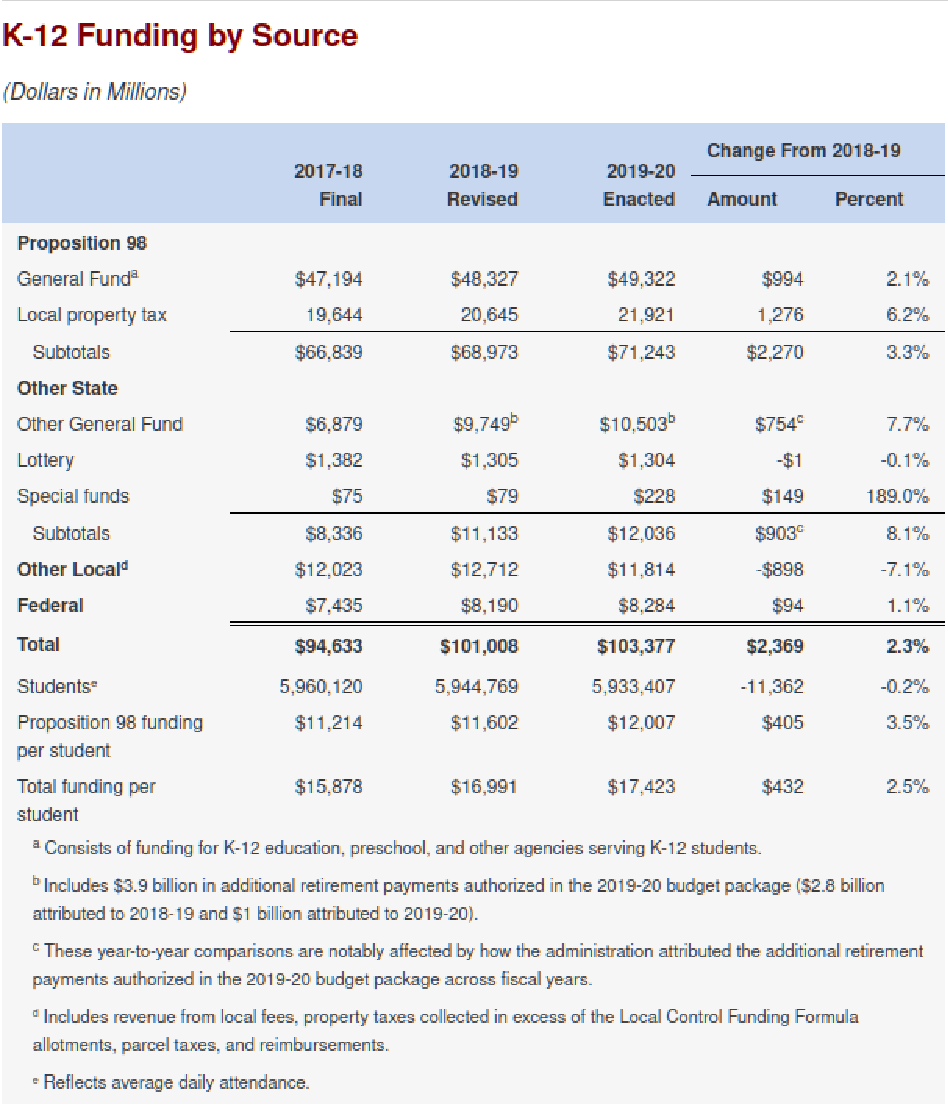
\includegraphics[width=0.9\textwidth]{2019-20_K-12_Funding_by_Source.pdf}\\ %chktex 8
  \footnotesize\raggedright\textcite{LAO2021}.
\end{figure}
The amount of the state budget that is allocated to K-12 is governed by Proposition 98. How Proposition 98 money is allocated to local educational agencies (LEAs) is calculated using a formula known as the Local Control Funding Formula (LCFF).\footnote{Currently, the LCFF funds transitional kindergarten and community colleges as well as public primary and secondary schools, so it ought to be known as funding grades TK-14. Appoximately 89\% of LCFF funding goes to grades TK-12.} LEAs include individual charter schools, county offices of education, and local public school districts. The total amount of funding for TK–14 is calculated using a formula enacted by voters in 1988, since modified, called Proposition 98. That proposition passed as a response to the notorious Proposition 13, which was enacted a decade earlier, and which decimated school funding. Prop. 98 was originally meant to be a minimum guaranteed funding level, but has evolved into a target to be met, i.e.~both a floor and a ceiling. The Legislative Analyst's Office (LAO), which serves as an independent, non-partisan research arm of the California Legislature in much the same way that the Congressional Research Service serves the U.S. Congress, calls Prop. 98 ``A Tale of Complexity''  and says that ``A Plethora Tests and Rules Govern the Minimum Guarantee'', and that ```[The] State Has Made Myriad Adjustments to the Proposition 98 Calculations'' \parencite[5]{LAO2017}.
\index{Proposition 98|)}
Undoubtedly LCFF is complex, but LCFF is more transparent, has fewer rules, is more equitable, and is more responsive to the needs of public school districts that have a high proportion of under-served students than its predecessor, the Revenue Limit System. The Revenue Limit System was also complex, but in a completely difference way because it had many separately funded programs, called categorical programs, each with their own set of requirements, rules, durations, and funding levels. Each passing year saw more programs being added to the set of categorical programs until the entire collection became so unwieldy and so inequitable that the need to replace it was felt by everyone.

The most succinct summary of how LCFF amounts are calculated is provided by the \textcite{CDE2023a}:
\begin{quotation}\noindent\SingleSpacing\vspace{-1\baselineskip}
  Funding entitlements under the LCFF consist of:
  \begin{enumerate}
    \item Grade span-specific base grants based on ADA, that reflect adjustments for grades K–3 class sizes and grades 9–12 (school districts with qualifying schools may receive a necessary small school (NSS) allowance in lieu of the base grants);
    \item Supplemental grants equal to 20 percent of the adjusted base grants multiplied by the LEA’s unduplicated percentage of English learners, income eligible for free or reduced-price meals, and foster youth pupils;
    \item Concentration grants equal to 65 percent of the adjusted base grants multiplied by an LEA’s percentage of unduplicated pupils above 55 percent;
    \item Two add-ons equal to the amounts school districts received in 2012–13 for the Targeted Instructional Improvement Block Grant and Home-to-School Transportation programs;
    \item An Economic Recovery Target add-on; and
    \item Beginning in 2022–23, an add-on for current year Transitional Kindergarten ADA.
    \item Base, supplemental, and concentration grants, as well as necessary small school allowances, receive cost-of-living adjustments as provided through the annual budget. Beginning in 2023–24, transportation related add-ons and the Transitional Kindergarten add-on will also receive cost-of-living adjustments.''
  \end{enumerate}
\end{quotation}

For the 2022-23 school year, a school\footnote{Loosely based on Discovery Prep which has only 428 students.} with 543 pupils total (181 TK–5 pupils per strand and 3 strands), of which 70\% are unduplicate pupils, and assuming the maximum size for a classroom with one teacher, the core LCFF calculation (adjusted grade-span base + supplemental + concentration) is as follows:\label{example_LCFF_calculation}\\\bigskip

\noindent\textbf{Adjusted base grant} \hfill{}(one-time adjustment + COLA + grade-span) \texttt{x} unduplicated count
\OnehalfSpacing%
\begin{verbatim}
TK–3: $10,119 × (127 pupils × 3 strands)        = $3,855,339
 4–5: $ 9,304 ×  (54 pupils × 3 strands)        = $1,507,248
\end{verbatim}
\noindent\textbf{Supplemental grant} \hfill(20\% of adjusted base grant) \texttt{x} unduplicated count
\OnehalfSpacing%
\begin{verbatim}
TK–3: 20% × $10,119 × (70% × 127 × 3)           = $  538,330
 4–5: 20% × $ 9,304 × (70% ×  54 × 3)           = $  210,270
\end{verbatim}
\noindent\textbf{Concentration grant} \hfill{}((\% over 55\%) \texttt{x} 65\% of adjusted base grant) \texttt{x} unduplicated count
\OnehalfSpacing%
\begin{verbatim}
TK–3: (70% - 55%) × (65% × $10,119) × 127 × 3   = $  375,895
 4–5: (70% - 55%) × (65% × $ 9,304) ×  54 × 3   = $  159,829
                                                  ==========
                                           total  $6,271,016
\end{verbatim}
\DoubleSpacing

\prettyref{fig:lcff_components} diagrams just the major components of the LCFF. It takes the Fiscal Crisis and Management Team's (FCMAT's) spreadsheet of 45 individual sheets to specify completely how the LCFF for a particular school or district is calculated \parencite{FCMAT2024}. The intricacies of LCFF funding are also covered in Chapter 3 of \textcite[35–58]{Aguinaldo.etal2022}.

\begin{figure}[htb]
  \caption[LCFF Components]{\textit{LCFF Components}}\label{fig:lcff_components}%
  \copyrightbox[b] {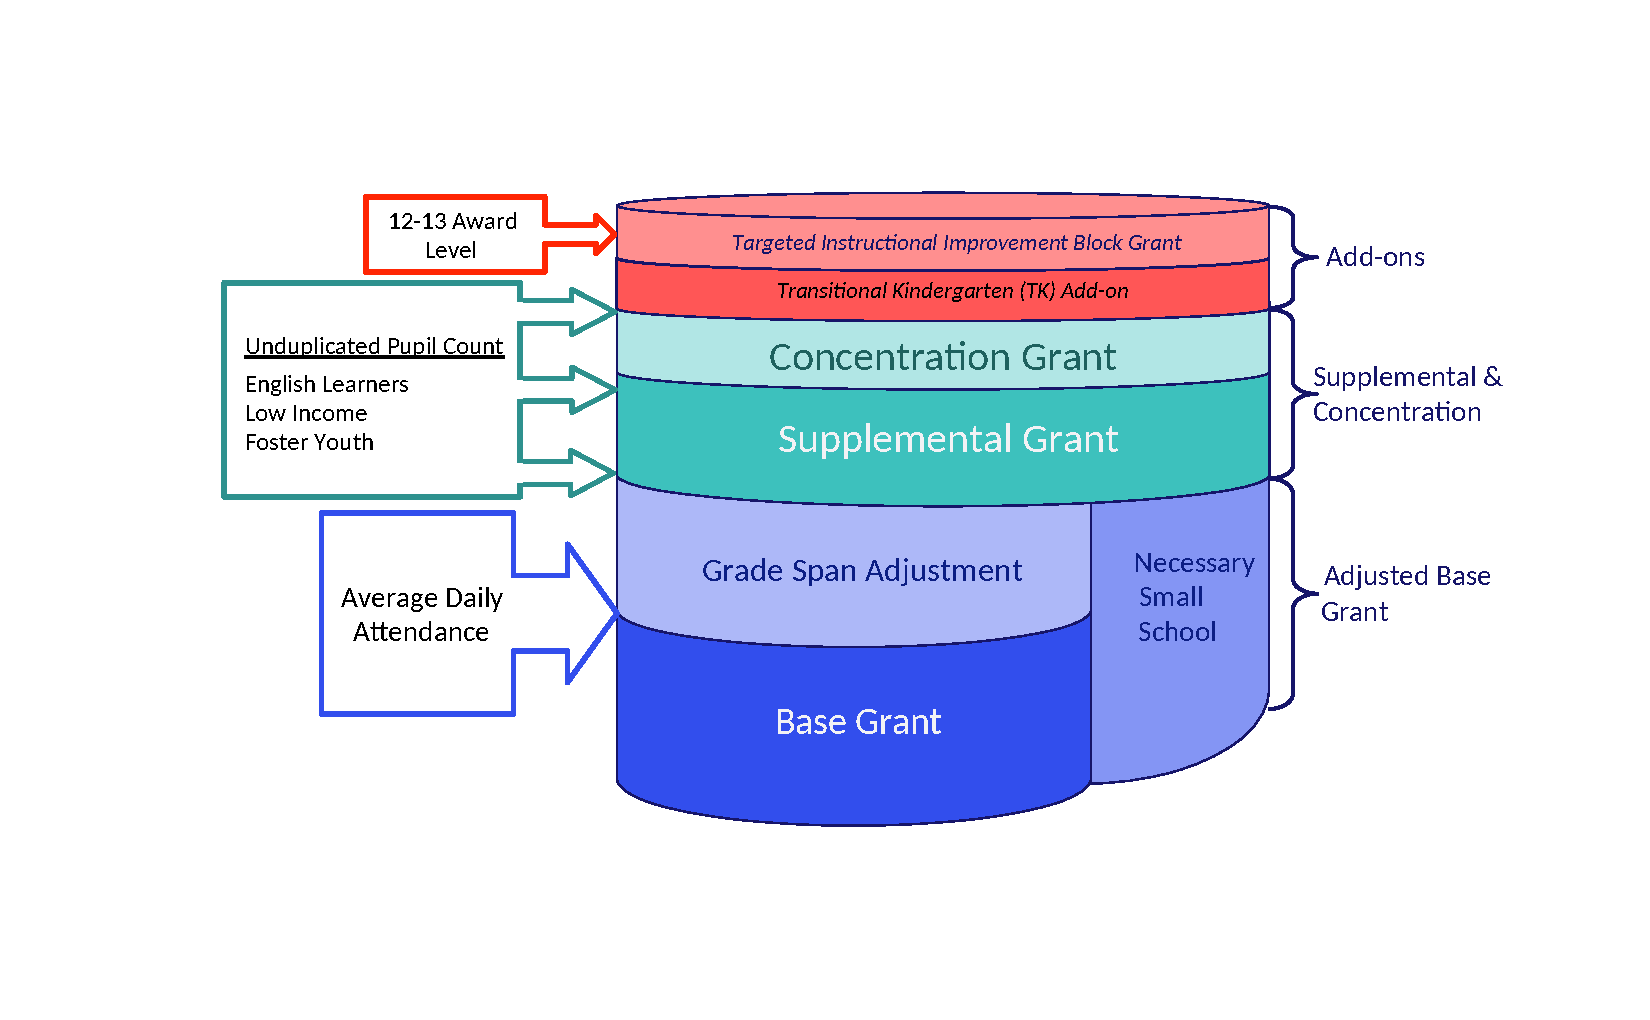
\includegraphics[scale=0.45] {LCFF_Components}}%
  {Adapted from ``Local Control Funding Formula Resources for School Districts and Charter Schools'' at \url{https://www.fcmat.org/PublicationsReports/LCFF-Calculator.xlsx}}
\end{figure}
\index{LCFF|)}

\index{Proposition 98|(}
As seen in \prettyref{fig:2019–20_K–12_Funding} on \pageref{fig:2019–20_K–12_Funding}, Proposition 98 funding accounts for nearly 70\% of California's K–12 funding, with the remainder coming from local property taxes and fees, and from various federal and state sources. This money is distributed to local educationa agencies (LEAs) which then distribute it to public school districts. Public school districts then distribute LCFF funds to charter schools located within their district. For community-funded districts (see below), charter schools represent a significan drain on their revenues.\footnote{For example, LASD sends \$10M to the Bullis Charter School (BCS) annually, equivalent to roughly 11\% of revenue.}
\index{Proposition 98|)}

Some districts are funded outside the LCFF system. These used to be called ``basic aid'' districts, but since the term is confusing, they are now called ``community funded'' districts. These are districts where their share of their county's annual property tax revenue is greater than their annual LCFF entitlement.\index{basic aid}\index{comunity funded} They get only ``basic aid'', i.e.~the constitutionally required minimum funding (the greater of \$120 per pupil or \$2,400 per district) from the state. For districts which are not community funded, the state contribution is the difference between a district's LCFF entitlement and its share of district property taxes. In other words, the state ensures that each district gets at least its LCFF entitlement, the total amount which is determined by Prop. 98.\footnote{An invaluable and comprehensive description of K-12 funding in California, for both public school districts and charter schools, can be found in an annual publication from School Services of California, Inc., e.g. \citetitle{Aguinaldo.etal2023}}.\index{K-12 funding!comprehensive description of (fn)}

\subsection{Budgets \& Interim Reports}\label{sec:budgets}\indent%

For a given fiscal year, the annual budget\index{budgets!annual} is the first of four important financial documents produced. Since budgets must be approved before the start of a fiscal year, budgets are actually produced and approved in the prior fiscal year.\footnote{Since a school's budget must be approved before the state's budget is finalized, it is a certainty that a school district's budget will need to be modified after it has been approved.} The next two financial documents are two (unaudited) interim reports,\index{budgets!interim reports} one in December, and another in March, which track how well the school or district is adhering to its approved annual budget, adjustments being allowed, and finally, after a certified public accountant has audited the school or district, a comprehensive annual financial report (CAFR)\index{budgets, audited}\index{Comprehensive Annual Financial Report (CAFR)} is produced in the fiscal year following the period it covers. State law requires that an independent auditor certify this retrospective account of the school or district's financial activity as being an accurate representation of the school's finances for the previous fiscal year.

\subsection{Local Control Accountability Plans (LCAPs)}\label{sec:lcaps}\indent%

\index{LCAP|(}
An important, recurring, non-financial report of a school district or a charter school is the Local Control Accountability Plan (LCAP).
\index{Local Control Accountability Plan (LCAP)} Although the LCAP is a three-year plan, it is updated annually. The focus of an LCAP is on the programs that a school district or charter school is going to implement, finance, and monitor that will allow the district or school to meet state goals. These goals are set periodically by the California Department of Education to ensure that students with the greatest needs are in fact served, and are in addition to the seven goals that the Legislature has set for charter schools in general.

Typically, LCAP goals remain the same over their three year lifespan, but their financing may change if the metrics used to measure progress toward achieving those goals are not showing progress. In unusual circumstances, how the goals are to be achieved might change. LCAPs are California's way of ensuring that all public schools, including charter schools, meet the same set of priorities or goals. Apparently, some LCAPs have been on the order of 500 pages long, although the norm is much less.

For each activity or group of activities, schools must indicate what goal is being met, if the goal includes increased services for disadvantaged student, how well the school or district has met that goal, and how much money has been allocated to achieving and reporting those goals. (The reality of what the Department of Education wants is an order of magnitude more complicated than this description, but it is accurate as far as it goes.)

Unlike budgets and CAFRs, LCAPs do not have to ``add up'', nor do they have to offer a complete financial picture, but they do have to be consistent with other financial data. Expenditures have to be budgeted, and the amounts in a school's budget must agree with what's in the LCAP\@. The charter or public school's board must approve an LCAP at the same time as it approves its annual budget. According to \textcite[81]{Aguinaldo.etal2022}, while no explicit approval of a charter school's LCAP is required, chartering authorities may revoke the charter for a school which repeatedly fails to improve student outcomes.
\index{LCAP|)}

\subsection{Comprehensive Annual Financial Reports}\label{sec:CAFRs}\indent%

\index{Comprehensive Annual Financial Report (CAFR)|(}
The final major source of financial data from charter schools is an annual, independently audited, financial statement called the Comprehensive Annual Financial Report (CAFR). These are sent to the California Department of Education (CDE) and to a charter's County Office of Education (COE) annually. They cover the previous fiscal year and are similar to annual budgets because they report the same information, but in a format suitable for computer processing. CAFRs are retrospective whereas budgets are prospective. The major difference between budgets and CAFRs is that CAFRs are independently audited and budgets are not. 
\index{Comprehensive Annual Financial Reports (CAFR)|)}

Similarly to bond underwriters, financial auditors are liable\index{financial liability!auditors} for ``omitting, misstating, or obscuring [items which] could reasonably be expected to influence decisions that the primary users make on the basis of those financial statements'' \parencite{Cayamanda2020}, and this requirement tends to increase the diligence of the auditors. However, potential liability does not always result in truly comprehensive financial statements; sometimes the lure of accounting fees overwhelms any misgivings, as was the case with Enron and Arthur Andersen in 2001. Errors and sloppiness may exist, but in general, fraud is thankfully rare, in part because fraud on the part of auditors would likely result in the loss of the auditor's license, effectively ending their business. 

\section{Charter School Financing}\label{sec:charter-school-financing}\indent%

\index{charter schools!financing of|(}
In California, charter schools are financed the same way as public schools are, from the same pot of money, using the same set of rules, except for one significant difference: how they finance facilities. Unlike public schools, charter schools have no taxing authority, so they cannot pass bond measures or parcel taxes. This lack of a taxing authority means that charter schools must either occupy existing public school facilities (possibly even displacing existing public school students) or seek grants and donations to fund non-district facilities, either leased or purchased. The federal government provides significant amounts of money for facilities through the Charter School Program \parencite[0–10]{NCSRC2020}. Likewise, the state of California provides support for charter school facilities \parencite[114]{Aguinaldo.etal2023}.

An in-depth analysis of charter school finances requires a broader lens than one used for public schools because, in addition to all of the financial dealings of traditional public schools, almost all of which also apply to charter schools, every charter school also has a large and immediate need for facilities that traditional public schools do not have. These needs potentially involve  bonds, loans, grants, construction, and the purchase, lease, or sale of real estate. Traditional public schools do issue several kinds of bonds, levy parcel taxes, and buy real estate on which they build schools, but they do so infrequently. Usually public schools have done this years ago, but new charter schools have an immediately and reoccurring need for facilities. They face these needs once when they start up, and whenever they outgrow their facilities because of increased enrollment. The needs of charter schools for facilities and the financing associated with obtaining those facilities is more pressing, more immediate, and more common than the corresponding needs of traditional public schools whose enrollment does not fluctuate as much.\footnote{Usually a public school district sees a change in enrollment because of significant demographic changes like immigration or emigration, birth rate increases or declines. Charter schools can see large enrollment changes absent any demographic change, even if the total number of students residing in a district stays the same. In some instances, increased enrollment in charter schools comes from public school students switching from the public school system to charter schools. This is what is happening to Oakland, CA and it produces simultaneous but opposite changes in enrollment.}
\index{charter schools!financing of|)}

\subsection{Charter School Financial Documents}\label{sec:charter-financial-docs}\indent%

The challenge for this inquiry will be to organize the financial documents and data collected so that gaps and anomalies can be identified, interesting and valid comparisons can be made with public schools and other charter schools, and the flows of money in and out of Rocketship can be identified. One way of organizing charter school data is chronologically from when they appear.

\prettyref{tab:charter-fin-docs}, summarizes the official, publicly available, and required financial reports about charter school finances, in chronological order. Note that budgets, interim reports, LCAPs, and CAFRs are also required of public schools. 

\begin{table}[ht]
  \centering\small%
  \caption[Charter School Financial Documents]{\textit{Charter School Financial Documents}}\label{tab:charter-fin-docs}%
  \begin{tabular}{llll}
    \toprule%
    \textbf{Name}  & \textbf{Description} & \textbf{Frequency} & \textbf{When} \\
    \midrule%
    Initial Petition  & Comprehensive description    & Once           & Before opening \\
    Renewal Petitions & Similar to initial petition  & Every 5 years  & Years 5, 10, 15, \ldots \\
    Budget            & Complete financial plan      & Annually       & Before June 15\textsuperscript{th} \\
    LCAP              & How to meet state priorities & Every 3 years  & With budget\\
    Interim Reports   & Current spending             & Twice yearly   & December, March \\
    CAFR              & Audited financials           & Annually       & In the following year \\
    \bottomrule%
  \end{tabular}
\end{table}%
\index{charter schools!initial petition}%
\index{charter schools!renewal petition}%
\index{charter schools!budget}%
\index{charter schools!LCAP}%
\index{charter schools!interim reports}%
\index{charter schools!CAFR}

\index{charter schools!initial petition|(}
The first financial statement from a charter school is contained in their initial petition. The purpose of the initial petition is to provide an authorizer with data on the charter school's educational program, pupil outcomes, methods to measure these outcomes, the charter school's governance structure, methods of racial and ethnic balancing, teacher and student health and safety, and among other measures.\footnote{Ed. Code §47605 (c)(5)(A–O)} Subsequent charter school data makes their apprearance during the school year, and then finally when a certified audit is completed.
\index{charter schools!initial petition|)}

All of Rocketship's schools have both initial and renewal petitions. These are voluminous, but fortunately the financial part is only a small portion of the total number of pages. In addition, a petition may have a corresponding staff report prepared by authorizers which evaluates the petition. These documents, and the others mentioned above are reviewed in the sections which follow.

\newpage
\subsubsection{Petitions \& Renewals}\label{sec:cs-petitions-renewals}\indent%

\index{charter schools!initial petition!required elements|(}
Before a charter school may legally begin operations, they must present to a chartering authority a petition which must contain certain required elements, and that petition must be accepted (with or without stipulations.) The absence of one of these elements is grounds for denying the charter's petition to operate. For example, what is the intent of the charter school? How is the charter school going to measure its success or failure? What population is it targeting? And, what are its financial projections? 

One of the required elements of any petition is a financial projection. Although no one expects a charter school (or any public school district for that matter) to prepare and adhere to a budget that exactly matches what's been projected, budgets are expected to be a reasonable approximation of future revenues and expenses.
\index{charter schools!initial petition!required elements|)}

\index{charter schools!petitions!publicly available|(}
Petitions run anywhere from a hundred or so pages to over a thousand and they contain a wealth of financial data. Fortunately, these documents are all publicly available and could, if needed, be the subject of a California Public Records Act (CPRA) request.\index{California Public Records Act (CPRA)} The CPRA is the California equivalent of the federal Freedom of Information Act (FOIA)\index{Freedom of Information Act (FOIA)}. Many of the documents mentioned in this dissertation are available from the California Departments of Education and Finance, or from the Santa Clara County Office of Education.\footnote{Since these documents are required to be publicly available and may be freely copied, no copyright is applicable.}
\index{charter schools!petitions!publicly available|)}

\index{Rocketship!annual financial statement|(} 
\index{Rocketship!501(c)(3) non profit|(} 
Since Rocketship schools are all operated by a single entity, (currently) Rocketship Education, DBA Rocketship Public Schools, a 501(c)(3) non-profit, their financial statements and those of their affiliates are rolled up into a single document, for example, ``Rocketship Education, Inc. and Its Affiliates, Consolidated Financial Statements and Supplementary Information, Year Ended June 30, 2022
(with Summarized Financial Information for the Year Ended June 30, 2021)''.  Every school is included in this single document, as are separate Launchpad Development LLC's that actually own the facilities leased to individual schools, plus two divisions provide specialized services. % chktex 36a
\index{Rocketship!501(c)(3) non profit|)} 
\index{Rocketship!annual financial statement|)} 

\subsubsection{Authorizer Staff Reports}\label{sec:cs-staff-reports}\indent%

\index{charter schools!petitions!staff reports|(}
Another set of documents that are related to initial and renewal petitions are the staff reports which usually accompany the agenda item which evaluates the charter school's petition in view of approval. In these reports, the authorizer's staff presents the findings and rationale for their recommendation to approve or not the petition of the charter school.
\index{charter schools!petitions!staff reports|)}

\subsubsection{Budgets,  Interim Reports, and CAFRs}\label{sec:budgets-etc}\indent%

\index{charter schools!annual filing requirement|(}
Once a charter has been granted the right to operate, it must file annually with the California Department of Education, just like public school districts, certain forms that detail its revenues and expenses. State law also mandates an annual audit by an independent accounting firm which charter schools must file with their County Office of Education. All together, these forms should provide a complete picture of a charter school's finances, and crucially, everything should be in agreement. Charters must approve and publish at a public meeting their annual budget, and they, just like traditional public schools, cannot spend unbudgeted money unless the governing board approves changes at a public meeting.
\index{charter schools!annual filing requirement|)}

\index{charter schools!interim reports|(}
Interim reports detail the differences between a school's budgeted revenue and expenses and actual revenue and expenses. Interim reports are filed twice each year in January (covering July - December) and April (covering January - March). As with the annual budget, deviations must be approved at a public meeting.
\index{charter schools!interim reports|)}

\index{charter schools!CAFR|(}
An independent public accounting firm audits the previous year's revenues and expenses and this becomes the definitive record of actual revenues and expenses. The textual version of their report is a consolitdated financial statement; the database on which it is based is a SACS (Standardized Account Code Structure) form and, when printed, is called the Comprehensive Annual Financial Report (CAFR)\index{Comprehensive Annual Financial Report. (CAFR)}  CAFRs are submitted to the school's County Office of Education (COE) to be forwarded to the California Department of Education. 
\index{charter schools!CAFR|)}

\subsubsection{LCAPs}\label{sec:cs-lcaps}\indent%

\index{charter schools!LCAP|(}
Like public schools in California, charter schools must submit an Local Control Accountability Plan (LCAP) that details how the charter school will meet the eight current state LCFF priorities regarding basic services and school conditions, state academic standards, parent engagement, student achievement, student engagement, school climate, access to a broad program of study, outcomes of a broad program of study \parencite[67–68]{Aguinaldo.etal2023}.

The intent of the LCAP is for schools to identify what they need to improve, paying particular attention to underserved groups, and how they plan to improve, and how they will measure improvement. 
\index{charter schools!LCAP|)}

\subsubsection{Board and Committee Supporting Material}\label{sec:board-committee-packets}\indent%

\index{Rocketship!board meetings|(}
Other sources of financial data are background material, presentations, and other documents that serve as input to board and committee meetings of both public schools and charter schools.  Rocketship publishes on their website, as required by California's Brown Act, agendas and supporting material for its board meetings and for certain committee meetings.\footnote{The Brown Act requires board-appointed committee meetings to be open to the public if they are standing meetings whose subject matter is within the jurisdiction of Rocketship's board, or if a majority of Rocketship's board are members of the committee.} Currently, Rocketship only provides on its web site meeting agendas and supporting material going back to February 2017. However, they had previously made material available going back to their founding in 2006, and that data was captured before it was deleted and will be part of this study.
\index{Rocketship!board meetings|)}

\section{Charter Schools and Real Estate}\label{sec:real-estate}\indent%

The last major financial topic of interest has to do with real estate. Since charter schools in California must obtain the facilities they plan to occupy before they receive any per-pupil state funding, real estate looms large in charter school finances. Charter schools have some leeway to choose whether to own or lease, and how to finance the acquisition of facilities, but in the end they must have or access to classrooms, play areas, administrative offices, and athletic fields for their students.

\subsection{Facilities Options}\label{sec:facilities-options}\indent%

\index{charter schools!facilities!options for|(}
As shown in \prettyref{tab:charter-facilities-options}, charter schools have three options: co-locate, lease, or purchase (with or without construction of bespoke facilities).

\begin{table}[ht]
  \small%
  \caption[Charter School Facilities Options]{\textit{Charter School Facilities Options}}\label{tab:charter-facilities-options}%
  \begin{tabular}{ll}
    \toprule%
    Option    & Description \\
    \midrule%If the school's facilities are leased, and SB740 funds are used to pay part of the rent, then appraisals and the amount of rent should be available from the administator of the SB740 program.
    Co-locate & \multirow[t]{2}{4.75in}{The charter school occupies ``reasonably equivalent'' facilities provided by 
                the public school district in which the charter school is located.}\\
                \\
    Lease     & The charter school occupies facilities that it leases.\\
    Own       & The charter school buys existing facilities or buys land and builds their own. \\
    \bottomrule%
  \end{tabular}
\end{table}
\index{charter schools!facilities!options for|)}

\index{charter schools!real estate documents|(}
Real estate transactions entail numerous, detailed legal documents, many of which are publicly available. If a charter school co-locates, then the terms have to be approved at a open meeting of the public school district in which the charter is located, and those are public documents. If the school's facilities are leased, and SB740 funds are used to pay part of the rent, then appraisals and the amount of rent should be available from the administator of the SB740 program. Ownership, with or without construction, has even more documents associated with the facility.
\index{charter schools!real estate documents|)}

\subsubsection{Co-Locating}\label{sec:co-locating}\indent%

\index{charter schools!facilities!co-location|(}
The least costly option for charter schools is to co-locate in an existing school. Proposition 39 and enabling regulations\footnote{Ed. Code §47614 et seq.  and 5 CCR § 11969.1} require that school districts furnish facilities for all in-district charter school students that are reasonably equivalent to those of students in the district in which the charter school resides. Facilities include regular and specialized classrooms, administrative offices, playgrounds, and athletic fields. It does not matter if the school district has unused space or not. It does not matter if the charter school grows in enrollment year over year. The requirement is rigid; school districts are required to furnish reasonably equivalent facilities under Proposition 39. However, districts and charter schools may enter into agreements outside of Proposition 39 concerning what facilities districts will provide to the charter school. Many charter schools choose the co-locating path, with or without a district's cooperation.

In theory co-locating is the least costly and most timely option for charter schools to obtain facilities, but often there is litigation over the extent or appropriateness of the facilities that the district provides. Sometimes these lawsuits drag on for years, often at a considerable expense for both the charter school and the public school district.
\index{charter schools!facilities!co-location|)}

\subsubsection{Leasing}\label{sec:leasing}\indent%

\index{charter schools!facilities!leasing|(}
Charter schools may lease their facilities from either a related party such as a 509(a)(3) supporting charity, or at arms length, from an unrelated party. The terms and length of leases vary. If the lessor is an unrelated party, the charter schools may take advantage of grants offered by the Charter School Finance Authority\footnote{Originally administered by the Department of Education; now administered by the California State Treasurer.} which are authorized by Ed. Code §47614.5 et seq. and CCR §10170\footnote{aka SB740} ``to offset annual on-going facility costs for charter schools that service a high-percentage of students eligible for free or reduced-price meals (FRPM) or located in a public elementary school boundary serving a similar demographic'' \parencite{CATreasurer2023}. The amount of the grant is the lesser of the school's ADA × \$1,420 or the annual rent × 75\%.\footnote{This is the basic calculation. As expected, there are variations and permutations, and these are enumerated in §6, Grant Award Calculations of the program's FAQ\@.} To be eligible, 55\% of a charter school's students must be eligible for free or reduced-price meals (FRPM) or be located in a public elementary school boundary serving a similar demographic \parencite[§1]{CATreasurer2023}.

If the charter school is leasing from a related party, usually SB740 grants are not available. However, the definition of \emph{related party} in this case does not include non-profit entities whose only business is supporting charter schools. For example, a non-profit charter school may lease a property from a related non-profit entity whose only business is owning and maintaining that property. This is the relationship that Rocketship Education has with the owners of the facilities they lease. The structure of Rocketship Education is diagrammed in \prettyref{fig:corporate-structure} on p.~\pageref{fig:corporate-structure}.
\index{charter schools!facilities!leasing|)}

\subsubsection{Owning}\label{sec:owning}\indent%

\index{charter schools!facilities!owning|(}
The third way of obtaining facilities is to own the needed facilities, or to have a related party own the facilities. These might be purchased, or the land purchased and facilities constructed. Most public school districts own their own facilities, but since these were likely bought and built using bond money derived from taxes, charter schools, lacking taxing authority, are unable to pay for their facilities this way.
\index{charter schools!facilities!owning|)}
\index{charter schools!facilities!financing of|(}
If a charter school's leadership decides they should own their own facilities, there are a number of ways they can go about this, as shown in \prettyref{tab:paying-for-facilities}.

\begin{table}[ht]
  \caption[Charter School Options for Paying for Facilities]{\textit{Charter School Options for Paying for Facilities}}%
  \label{tab:paying-for-facilities}%
  \begin{tabular}{ll}
    \toprule%
    \textbf{Option}    & \textbf{Source of Funds} \\
    \midrule%
    \protect\medskip%
    \multirow[t]{2}{1.25in}{Private grants or loans} & \multirow[t]{2}{4.25in}{Private entities (individuals or foundations) may make a grant or a loan to  a charter school.}\\\\ %
    \protect\medskip%
    Venture funds & \multirow[t]{2}{4.25in}{Venture Funds which ostensibly intend to make money often loan money to charter schools.}\\\\
    \protect\medskip%
    \multirow[t]{3}{1.25in}{Federal or state grants} & \multirow[t]{3}{4.25in}{Both the federal government and states have programs which offer funds that may be used to pay for existing facilities or for new construction.}\\\\\\
    \protect\medskip%
    Tax credits & \multirow[t]{2}{4.25in}{The federal government offers tax credits for investors whose investments meet
certain criteria.}\\\\
    Bonds & \multirow[t]{3}{4.25in}{Charter schools may use the commercial or municipal bond markets to obtain funds, but property or parcel taxes may not be used to pay them off.}\\\\\\
    \bottomrule%
  \end{tabular}
\end{table}

\subsubsection{Private Funding: Loans and Foundation Grants}\label{sec:private-funding}\indent%

Individuals or non-public entities often loan or give money to charter schools, including Rocketship. Some are outright grants; others are expected to be paid back; still others may be partially paid back and then forgiven. Each grant has its own set of terms and interest rate.

\subsubsection{Venture Funds}\label{sec:venture-funds}\indent%

The NewSchools Venture Funds\footnote{\url{https://www.newschools.org/}} and the Charter School Growth Fund\footnote{\url{https://chartergrowthfund.org/}} are two examples of venture funds that specialize in charter schools. Since it is unlikely that investors will invest in a fund that does not return a profit, a future investigation should establish exactly how these funds turn a profit.\footnote{It is interesting that none of the web sites of these funds mentions that fund's return on investment (ROI). The absence of any indication of a return on investment is either an innocent mistake or much more likely, an attempt at obfuscation.}

\subsubsection{Tax Credits}\label{sec:tax-credits}\indent%

Tax credits are often used as a source of funds to buy or construct facilities. For example, the New Markets Tax Credit (NMTC) is a 39\% tax credit, usable over seven years, available to those who make an investment in specified economically depressed neighborhoods. This 39\% tax credit is can be used to offset federal taxes on other investments. Note that the investment which generates the tax credit may itself also have a return. The NMTC is discussed in more detail in \prettyref{sec:NMTC} on p.~\pageref{sec:NMTC}.

\subsubsection{Bonds}\label{sec:bond-prospectuses}\indent%

All bonds are to some extent risky, some more than others, and purchasers of those bonds are compensated for taking on that risk by being paid interest on the amount borrowed. So, when a bond is issued, the terms (e.g. interest rate, repayment schedule, collateral, etc.) are described in great detail in a prospectus. These prospectuses, in addition to the terms, contain financial information relevant to assessing the risk associated with purchasing that bond. Bonds, after all, are loans, and when millions of dollars are being loaned, those making the loans want to be assured of getting paid back and paid back on time, particularly since charter schools are known to close abruptly.

Bond prospectuses can be mined for data that might not appear in petitions or financial statements because bond underwriters might be liable for representations or omissions in a prospectus which are material. This liability, of course, is not unlimited. If bond underwriters exercise due diligence or the misrepresentation is not material, the underwriters are probably not liable. Crucially, the definitions of \textit{material misrepresentation} and \textit{due diligence} depended on both statute and case law, so a bond underwriter can only make a reasoned guess at their exposure to liability. The result is that bond underwriters are likely to be more diligent than is absolutely necessary.
\index{charter schools!facilities!financing of|)}

\section{Other Data}\label{other-data}\indent%

\subsection{State and Federal Filings}\label{sec:state-federal-filings}\indent%

\index{California!FPPC Form 700, Statement of Economic Interests|(}
Two filings are of particular interest, one with the state, and one with the federal government: FPPC Form 700, Statement of Economic Interests, and IRS Form 990, Return of Organization Exempt from Income Tax. Both forms force the disclosure of personal financial information (Form 700) or personal financial information and business financial information (Form 990). 

Some officers of Rocketship may be required to submit annually to the California Fair Political Practices Commission (FPPC) Form 700, Statement of Economic Interests. This particular requirement of charter school officers is not settled law,\footnote{Rocketship's initial petition for Mateo Sheedy states that Form 700, Statement of Economic Interest, shall be filed by all board members, candidates for board membership, corporate officers, principals and assistant principals, among others.} but if Form 700 is filed, it will list the submitter's assets and income that are related to the position they hold in Rocketship Education or Launchpad Development. The intent is to prevent related-party transactions by enumerating an officer's economic interests so that a school can avoid doing business with entities that might indirectly benefit an officer. (Of course, direct benefit is absolutely not permitted, and if it occurs, is graft.)  
\index{California!FPPC Form 700, Statement of Economic Interests|)}

\index{Internal Revenue Service Form 990|(}
The federal Internal Revenue Service grants income tax exemptions to organizations that meet the requirements of §501(c)(3) of the  Internal Revenue Code.\footnote{26 USC 501, i.e. Title 26, Subtitle A, Chapter 1, Subchapter F Part I § 501(c)(3)} These organizations must file Form 990 annually that provides some minimal financial data.\footnote{Tax returns of for-profit organizations are not public documents and their contents do not have to be disclosed; however, in order to sell stock to the public, i.e.~to be listed on a stock exchange, firms are required to publish various financial documents, which like bond prospectuses, are required to be informative and complete.} %chktex 36
\index{Internal Revenue Service Form 990|)}

\subsection{Curated Social Media}\label{sec:curated-social-media}\indent%

\index{social media|(}
Some web sites maintain data related to Rocketship. For example, the \textit{Scoop.It!} topic, `Charter Schools \& ``Choice'': A closer look'\footnote{\url{https://www.scoop.it/topic/charter-choice-closer-look}} is devoted to charter schools in general, but also has material specifically on Rocketship. The now extinct web site, ``Stop Rocketship Education Now!''\footnote{\url{http://www.stoprocketship.com}} was created and maintained by community volunteers. Web scrapes of both of these sites were obtained in case they were deleted (which in fact was the case with ``Stop Rocketship Education Now!'').
\index{social media|)}

\section{Gaps and Anomalies}\label{sec:gaps-anomalies}\indent%

\index{gaps and anomalies|(}
No financial statement is perfect, and not all are in agreement. But there is a difference between an innocent mistake or omission, and one designed to deceive and mislead. Triangulation can be used to capture gaps and anomalies.
\index{gaps and anomalies|)}

\subsection{Triangulation}\label{sec:triangulation}\indent%

\index{triangulation|(}
Triangulation is the process of comparing different documents from different sources that contain overlapping topics. The greater the number of sources, the greater the chance of catching gaps and anomalies.

One might ask questions such as:
\begin{itemize}
  \item Does everything add up? 
  \item Are there important, missing documents? 
  \item How much do these gaps or anomalies matter? 
  \item Are the oddities long-standing or fleeting? 
\end{itemize}
Examples of triangulation might be comparing Rocketship's LCAPs to their budget, or comparing IRS Form 990 data to their audited financial statements.
\index{triangulation|)}

%%% Local Variables:
%%% mode: latex
%%% TeX-master: "Rocketship_Education-An_Exploratory_Public_Policy_Case_Study"
%%% End:

